%!TEX root = ./template-skripsi.tex

\subsection{Sprint 6 Report}
Berikut merupakan report dari sprint ke-5 yang dilakukan pada tanggal 29 juni - 5 juli 2022.

\begin{table}[H]
	\caption{\textit{Sprint-6 backlog}}
	\label{sprint6_backlog}
	\begin{tabular}{@{} |p{0.5cm}|p{5cm}|p{5cm}|p{2cm}| @{}}
		\hline
		\textbf{No} & \textbf{\textit{Story}} & \textbf{\textit{Task}} & \textbf{\textit{Status}} \\
		\hline
		1 & & Implementasi controller delete kematian ikan & Complete\\
		\cline{1-1}\cline{3-4}
		2 & & Membuat view rekap kematian ikan perbulan & Complete\\
		\cline{1-1}\cline{3-4}
		\hline
	\end{tabular}
\end{table}

\begin{enumerate}[1.]



\item \textbf{Implementasi API fetch list kematian ikan berdasarkan kolam}

Implementasi controller API fetch list kematian ikan berdasarkan kolam, berikut merupakan source code controller API fetch list kematian ikan berdasarkan kolam.

\begin{lstlisting}
# fishapi/database/fishdeath.py

def get(self):
        try:
            url = url_for('fishdeathimageapidummy', _external=True)
            pipeline = [
                {'$lookup': {
                    'from': 'pond_activation',
                    'let': {"pondid": "$_id"},
                    'pipeline': [
                        {'$match': {'$expr': {'$and': [
                            {'$eq': ['$pond_id', '$$pondid']},
                            {'$eq': ['$isFinish', False]},
                        ]}}},
                        {"$lookup": {
                            "from": "fish_death",
                            "let": {"activationid": "$_id"},
                            "pipeline": [
                                {'$match': {'$expr': {'$and': [
                                    {'$eq': ['$pond_activation_id',
                                             '$$activationid']},
                                ]}}},
                                {'$lookup': {
                                    'from': 'fish_log',
                                    'let': {"fish_death_id": "$_id"},
                                    'pipeline': [
                                        {'$match': {
                                            '$expr': {'$and': [
                                                {'$eq': ['$fish_death_id',
                                                         '$$fish_death_id']},
                                                {'$eq': ['$type_log',
                                                         'death']},
                                            ]}
                                        }},
                                        {"$project": {
                                            "created_at": 0,
                                            "updated_at": 0,
                                        }}
                                    ],
                                    'as': 'fish'
                                }},
                                {"$addFields": {
                                    "image_link": {"$concat": [url, "/", {"$toString": "$_id"}]}
                                }},
                                {"$project": {
                                    "pond_id": 0,
                                    "pond_activation_id": 0,
                                    "created_at": 0,
                                    "updated_at": 0,
                                }}
                            ],
                            "as": "fish_death_list",
                        }},
                        {"$project": {
                            "pond_id": 0,
                            "feed_type_id": 0,
                            "created_at": 0,
                            "updated_at": 0,
                        }}
                    ],
                    'as': 'pond_activation_list'
                }},
                {"$addFields": {
                    "pond_activation": {"$first": "$pond_activation_list"},
                }},
                {"$project": {
                    "location": 0,
                    "shape": 0,
                    "material": 0,
                    "length": 0,
                    "width": 0,
                    "diameter": 0,
                    "height": 0,
                    "image_name": 0,
                    "pond_activation_list": 0,
                    "updated_at": 0,
                    "created_at": 0,
                }}
            ]
            ponds = Pond.objects.aggregate(pipeline)
            list_ponds = list(ponds)
            response = json.dumps(list_ponds, default=str)
            return Response(response, mimetype="application/json", status=200)
        except Exception as e:
            response = {"message": str(e)}
            response = json.dumps(response, default=str)
            return Response(response, mimetype="application/json", status=400)
\end{lstlisting}

Kode yang diberikan adalah sebuah method get yang ada di dalam sebuah class. Method ini menerima request GET untuk mengambil data dari MongoDB database.

Berikut adalah langkah-langkah yang dilakukan oleh method get:

\begin{enumerate}[a.]
\item Membuat URL dari fishdeathimageapidummy dengan menggunakan url\_for dan menyimpannya ke dalam variabel url.
\item Membuat sebuah pipeline untuk melakukan aggregate query pada collection Pond.
\item Pada pipeline tersebut, melakukan lookup terhadap collection pond\_activation dengan menggunakan field \_id dari collection Pond sebagai input.
\item Pada hasil lookup pertama, mencocokkan nilai dari field isFinish yang bernilai False.
\item Pada hasil lookup kedua, mencocokkan nilai dari field pond\_activation\_id yang sama dengan \_id dari hasil lookup pertama.
\item Pada hasil lookup ketiga, mencocokkan nilai dari field fish\_death\_id yang sama dengan \_id dari hasil lookup kedua dan type\_log yang bernilai death.
\item Melakukan projeksi untuk mengambil field-field tertentu yang dibutuhkan dan mengecualikan beberapa field yang tidak dibutuhkan.
\item Menyimpan hasil query dalam variabel ponds.
\item Mengubah hasil query menjadi sebuah list dan mengubahnya menjadi JSON dengan menggunakan json.dumps.
\item Membungkus hasil JSON kedalam sebuah response dengan menggunakan Response.
\item Jika terdapat exception, maka akan membuat sebuah response dengan pesan error dan mengembalikan response tersebut.
\item Inti dari kode ini adalah melakukan sebuah aggregate query pada collection Pond dengan menggunakan beberapa lookup dan projeksi untuk mengambil data yang dibutuhkan dan menyajikan hasil query dalam bentuk JSON.
\end{enumerate}


Berikut merupakan hasil test request dari API get list kematian ikan.

cURL:

\begin{lstlisting}
curl --location 'http://jft.web.id/fishapi/api/fishdeath'
\end{lstlisting}

response json:

\begin{lstlisting}
[
  {
    "_id": "62a62163e445ffb9c5f746f3",
    "id_int": 4,
    "alias": "charlie",
    "build_at": "2022-06-13 00:24:51.473000",
    "isActive": false
  },
  {
    "_id": "625d7033a9a73e090c65cda2",
    "id_int": 3,
    "alias": "beta",
    "build_at": "2022-04-18 21:05:39.608000",
    "isActive": true,
    "pond_activation": {
      "_id": "62b6b2f1a8a50041ee6350a4",
      "isFinish": false,
      "fish": [
        {
          "lele": 100
        },
        {
          "patin": 200
        }
      ],
      "isWaterPreparation": false,
      "water_level": 100,
      "total_fish_harvested": 0,
      "total_weight_harvested": 0,
      "activated_at": "2022-06-25 14:02:09.881000",
      "fish_death_list": []
    }
  },
  {
    "_id": "625d7026a9a73e090c65cda1",
    "id_int": 2,
    "alias": "alpha",
    "build_at": "2022-04-18 21:05:26.183000",
    "isActive": true,
    "pond_activation": {
      "_id": "62af4c24f6a3ffba25a6be6a",
      "isFinish": false,
      "fish": [
        {
          "lele": 100
        },
        {
          "patin": 200
        }
      ],
      "isWaterPreparation": false,
      "water_level": 1.34,
      "total_fish_harvested": 0,
      "total_weight_harvested": 0,
      "activated_at": "2022-06-19 23:17:40.501000",
      "fish_death_list": [
        {
          "_id": "62b9adfa793e0f39dbaa1739",
          "fish_death_amount": [
            {
              "lele": 10
            },
            {
              "patin": 20
            }
          ],
          "image_name": "Mass-fish-death-Menindee_1656335866.jpeg",
          "diagnosis": "mati karena sakit",
          "image_link": "http://127.0.0.1:5000/api/fishdeath/image/62b9adfa793e0f39dbaa1739"
        }
      ]
    }
  },
  {
    "_id": "62a955888911334402ddb3b3",
    "id_int": 5,
    "alias": "delta",
    "build_at": "2022-06-15 10:44:08.180000",
    "isActive": false
  },
  {
    "_id": "62ada3ff1dc3a711668e7ca3",
    "id_int": 7,
    "alias": "epsilon",
    "isActive": false,
    "build_at": "2022-06-18 17:07:59.396000"
  }
]
\end{lstlisting}

\item \textbf{Membuat view rekap kematian ikan perbulan}
\begin{figure}[H]
	\centering
	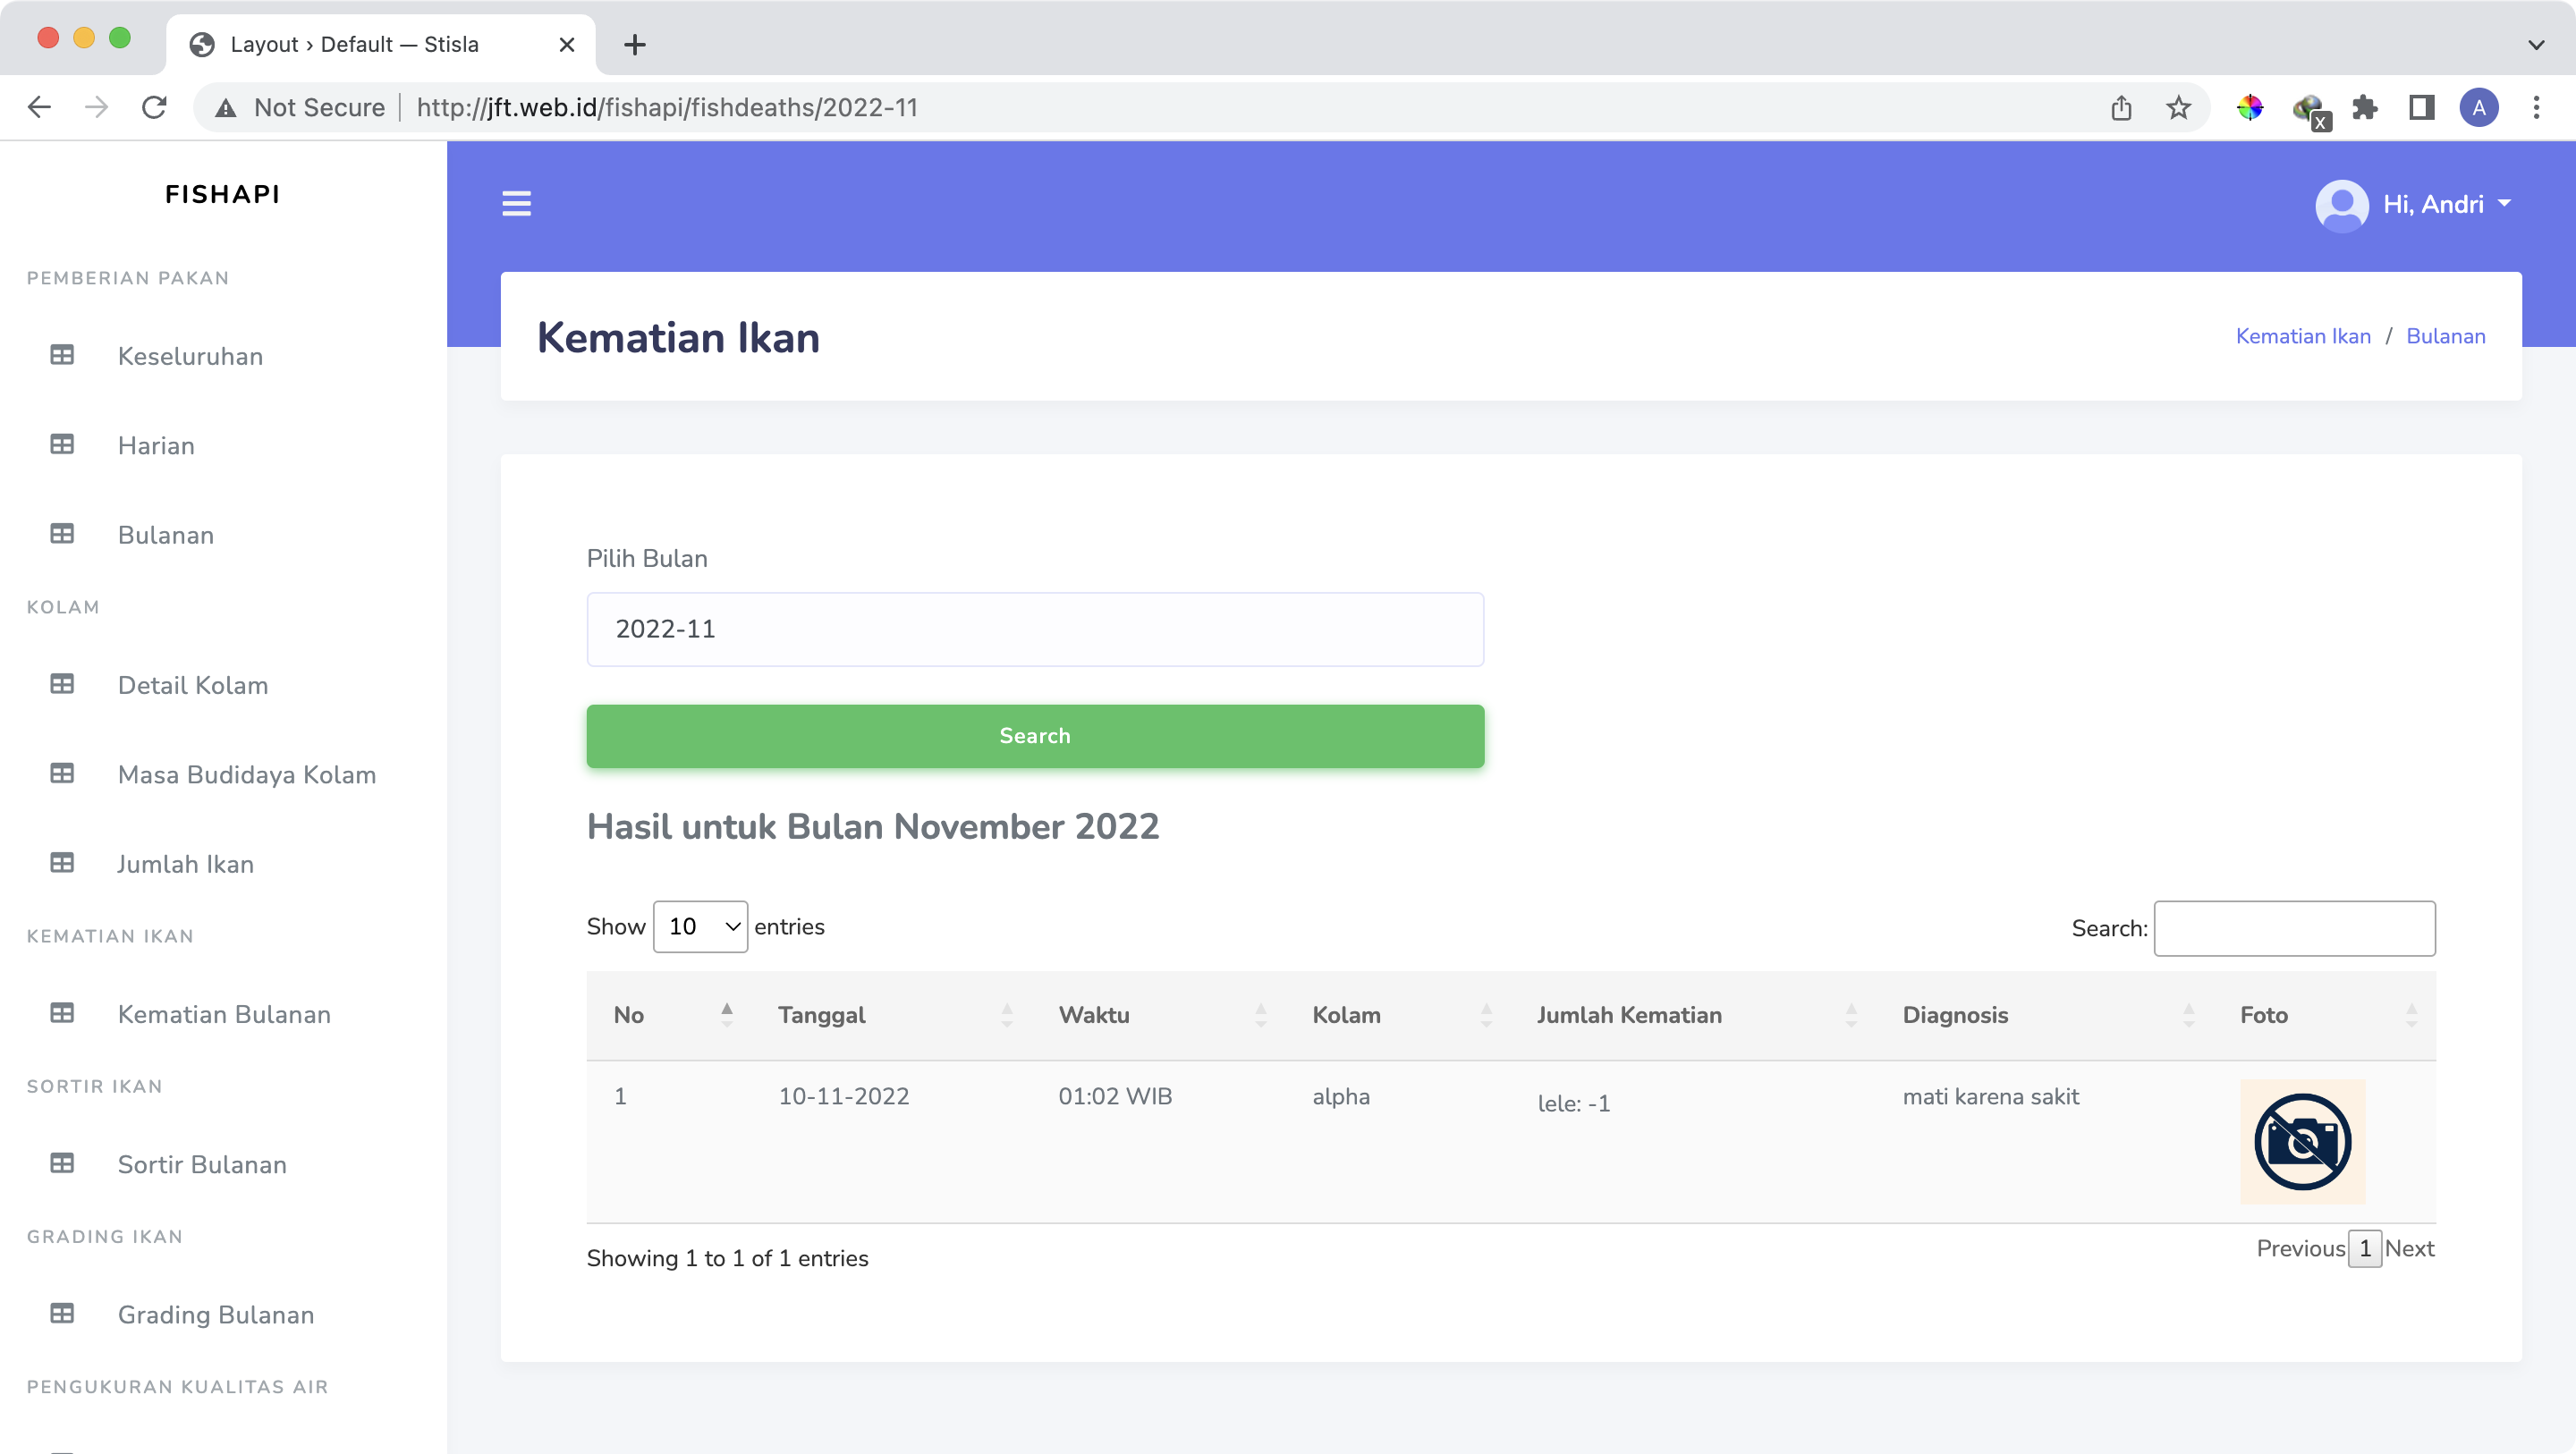
\includegraphics[width=1\textwidth]{gambar/Sprint05/view/view_kematian_bulanan}
	\caption{View list kematian perbulan}
	\label{fig:view_list_kematian_bulanan}
\end{figure}




\end{enumerate}